\documentclass{article}
\usepackage[utf8]{inputenc}
\usepackage{algorithm}
\usepackage{algpseudocode}
\usepackage{tikz}
\usetikzlibrary{automata,topaths}
\usepackage{pgfplots, pgfplotstable}
\usepackage{listings}
\lstset{language=Python}

\title{MC886 - Machine learning \\ Exercise 1}
\author{Rafael Almeida Erthal Hermano\\RA 121286}
\date{March 2014}

\begin{document}

\maketitle
\newpage

\section{KNN results without PCA}
\begin{table}[h]
\begin{tabular}{cl}
    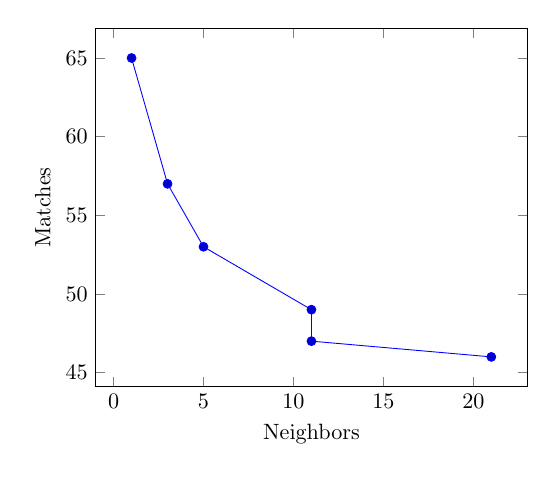
\begin{tikzpicture}[scale=0.8]
    \begin{axis}[xlabel=Neighbors, ylabel=Matches]
        \addplot coordinates {
            (1, 65 )
            (3, 57 )
            (5, 53 )
            (11, 49 )
            (11, 47 )
            (21, 46 )
        };
    \end{axis}
    \end{tikzpicture}
 &
    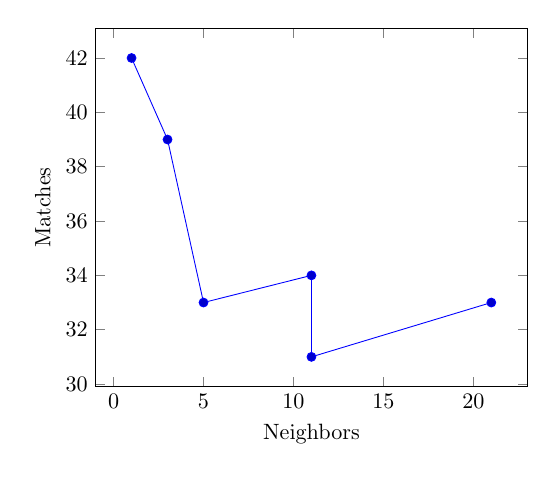
\begin{tikzpicture}[scale=0.8]
    \begin{axis}[xlabel=Neighbors, ylabel=Matches]
        \addplot coordinates {
            (1, 42 )
            (3, 39 )
            (5, 33 )
            (11, 34 )
            (11, 31 )
            (21, 33 )
        };
    \end{axis}
    \end{tikzpicture}
\end{tabular}
\end{table}

\section{KNN results with PCA reduced to 100 dimensions}
\begin{table}[h]
\begin{tabular}{cl}
    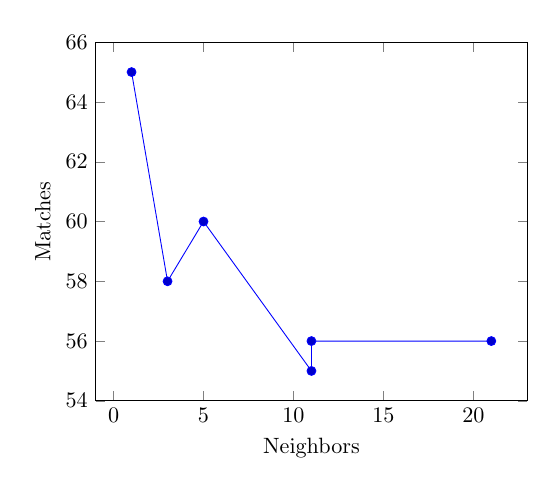
\begin{tikzpicture}[scale=0.8]
    \begin{axis}[xlabel=Neighbors, ylabel=Matches]
        \addplot coordinates {
            (1, 65 )
            (3, 58 )
            (5, 60 )
            (11, 55 )
            (11, 56 )
            (21, 56 )
        };
    \end{axis}
    \end{tikzpicture}
 &
    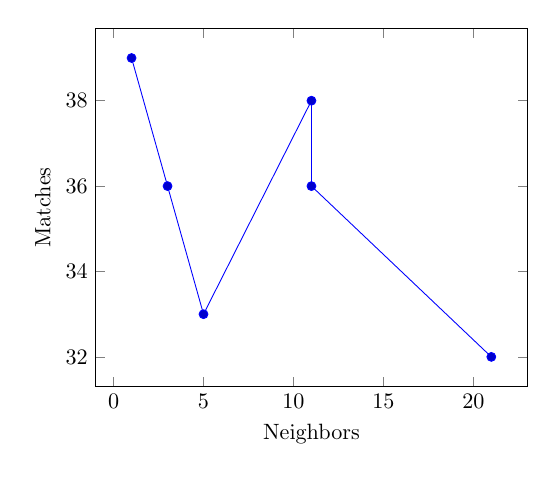
\begin{tikzpicture}[scale=0.8]
    \begin{axis}[xlabel=Neighbors, ylabel=Matches]
        \addplot coordinates {
            (1, 39 )
            (3, 36 )
            (5, 33 )
            (11, 38 )
            (11, 36 )
            (21, 32 )
        };
    \end{axis}
    \end{tikzpicture}
\end{tabular}
\end{table}

\section{KNN results with PCA reduced to 40 dimensions}
\begin{table}[h]
\begin{tabular}{cl}
    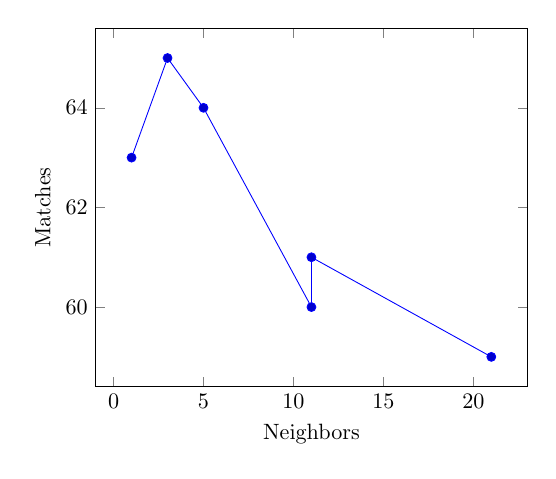
\begin{tikzpicture}[scale=0.8]
    \begin{axis}[xlabel=Neighbors, ylabel=Matches]
        \addplot coordinates {
            (1, 63 )
            (3, 65 )
            (5, 64 )
            (11, 60 )
            (11, 61 )
            (21, 59 )
        };
    \end{axis}
    \end{tikzpicture}
 &
    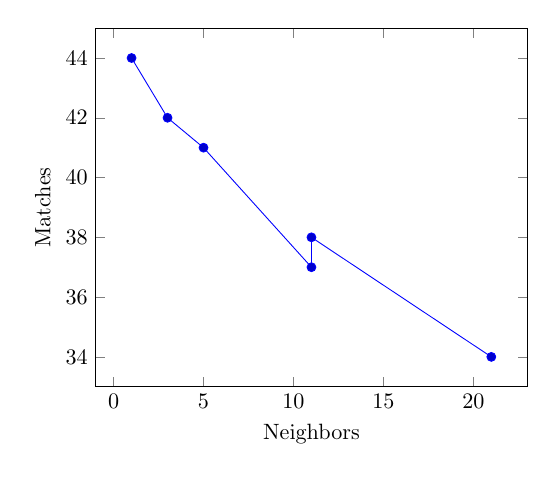
\begin{tikzpicture}[scale=0.8]
    \begin{axis}[xlabel=Neighbors, ylabel=Matches]
        \addplot coordinates {
            (1, 44 )
            (3, 42 )
            (5, 41 )
            (11, 37 )
            (11, 38 )
            (21, 34 )
        };
    \end{axis}
    \end{tikzpicture}
\end{tabular}
\end{table}

\end{document}